\chapter{PRIMER}
\section{Títol de la secció}
adf\\
\newline
sfsdfasfd
Per inserir equacions, recomano utilitzar un \href{https://www.codecogs.com/latex/eqneditor.php}{servei web} o bé un programa com, \href{https://www.codecogs.com/latex/eqneditor.php}{EqualX}. Fan la feina d'escriure equacions molt intuïtiva amb la seva interfície gràfica, després només cal copiar i enganxar el codi que generen. \\
$1=\sin b$\\
$x = a_0 + \frac{1}1=\sin b{a_1 + \frac{1}{a_2 + \frac{1}{a_3 + a_4}}}$\\
L'entorn \verb|equation| crea equacions enumerades que es poden etiquetar i referenciar on es desitgi:
%  Comentari per evitar començar un nou paràgraf
\begin{equation}\label{eq:pythagoras}
a^2 + b^2 = c^2
\end{equation}
L'equació \ref{eq:pythagoras} és el Teorema de Pitàgores.\\
%  this commented blank line prevents start of a new paragraph
Podeu utilitzar \verb|\eqref| per posar parèntesis al voltant de les referències a les equacions: \eqref{eq:pythagoras}.
%
\\Per mostrar equacions sense números utilitzeu \verb|equation*|:
%
\begin{equation}\label{eq:suma}
2 + 2 = 4 
\end{equation}
Per emmarcar una equació podem fer servir \verb|\boxed{equació}|:
\begin{equation*}
\boxed{E=mc^2}
\end{equation*}
Per evitar que les lletres quedin en italic (inclinades), escriure \verb|\mathrm{equació aquí}|. Per negreta, \verb|\textbf|, \textbf{text en negreta}.
\begin{equation*}
\mathrm{E=mc^2}
\end{equation*}
%
%
També podem inserir equacions enmig d'una línia com per exemple \(x^2 + y^2 = z^2\) aquesta equació, o bé $E=mc^2$ aquesta altra.
\begin{align*}
  f(x) &= x^2\\
  g(x) &= \frac{1}{x}\\
  F(x) &= \int^a_b \frac{1}{3}x^3
\end{align*}
També tenim l'opció de mostrar matrius, cal inicialitzar el mode matemàtic, ho podem fer cridant equation:
\begin{equation*}
	\begin{matrix}
		1 & 0\\
		0 & 1
	\end{matrix}
\end{equation*}
O millor:
    \[\begin{bmatrix}
        a & b \\
        c & d
    \end{bmatrix}\] 
\\
%
Per fòrmules multilínia, utilitzeu \verb|align| or \verb|align*|:
%
\begin{align}
e^{i\pi} & = \cos(\pi) + i\sin(\pi) \notag \\
         & = -1 .
\end{align}
% Per defecte les imatges salten de pàgina automàticament si no caben en una pàgina, i l'espai s'omple amb text. 
%Si es posa l'asterisc s'evita que s'enumeri

%
%Comentaris per evitar el tab
%
Vegeu \ref{fig:fs_mi} i \ref{fig:three_graphs}
%
Explicat com mostrar equacions i algunes opcions per això, anem a mostrar més exemples d'equacions:
Alguns caràcters , 
%, \beta, \Beta, \gamma, \Gamma, \pi, \Pi, \phi, \varphi, \mu, \Phi:
%
Fòrmula trigonomètrica:
\begin{equation*}
	\cos (2\theta) = \cos^2 \theta - \sin^2 \theta
\end{equation*}
Límit:
\begin{equation*}
	\lim\limits_{x \to \infty} \exp(-x) = 0
\end{equation*}
Operador:
\begin{equation*}
	a \bmod b
\end{equation*}
Potències:
\begin{align*}
	k_{n+1} = n^2 + k_n^2 - k_{n-1} \\
	n^{22} \\
	f(n) = n^5 + 4n^2 + 2 |_{n=17}
\end{align*}
Altres:
\begin{equation*}
	\frac{n!}{k!(n-k)!} = \binom{n}{k} \\
\end{equation*}
\begin{equation*}
	\int y\, \mathrm{d}x \\
\end{equation*}
\begin{equation*}
	\frac{\mathrm d}{\mathrm d x} \left( k g(x) \right) \\
\end{equation*}
\\
Per insertar una gràfica, programar-la amb Python amb:
%
\begin{lstlisting}
import matplotlib.pyplot as plt
# use LaTeX fonts in the plot
plt.rc('text', usetex=True)
plt.rc('font', family='serif')
# get the figure
f = plt.figure()


inicial = 5000
interes = 0.15

x = [1,2,3,4,5,6,7,8,9,10,11,12,13,14,15,16,17,18,19,20]
y = [1,2,3,4,5,6,7,8,9,10,11,12,13,14,15,16,17,18,19,20]
for i in range(15):
    y[i]=inicial*pow((1+interes), x[i])


# set labels (LaTeX can be used)
plt.title(r'\textbf{Mutual Information Feature Selection}', fontsize=11)
plt.xlabel(r'\textbf{Best K features}', fontsize=11)
plt.ylabel(r'\textbf{AUC Score on split11 Dataset}', fontsize=11)

plt.plot(x,y, label='Exponential')
plt.legend(loc='upper left')
# plt.grid()
plt.show()

# save as PDF
f.savefig("fs_mi.pdf", bbox_inches='tight')
\end{lstlisting}
El resultat:
\begin{figure}[H]
\centering
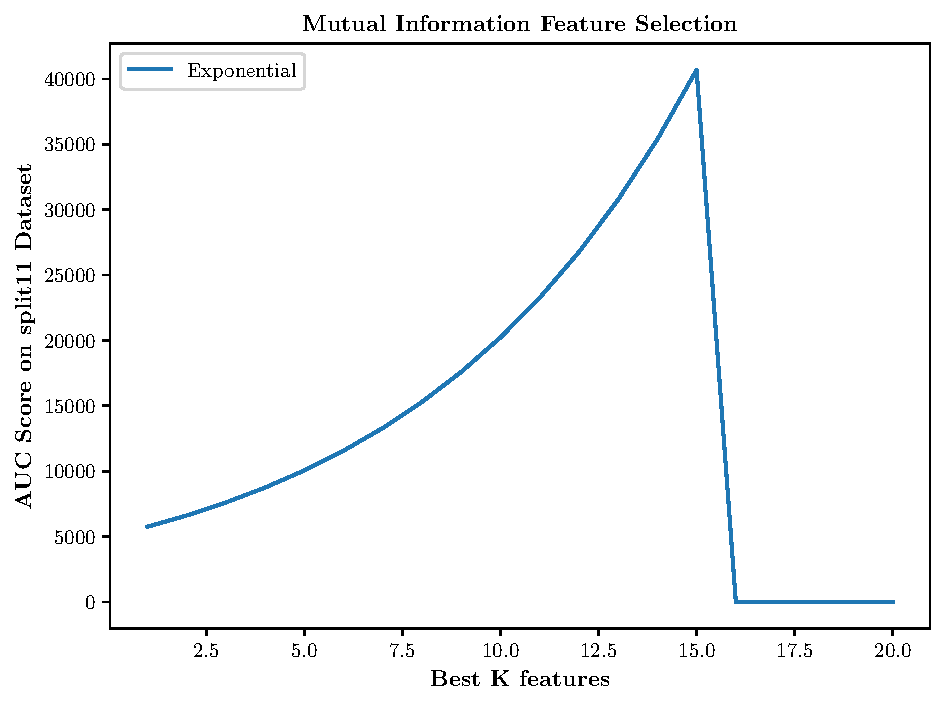
\includegraphics[scale=0.75]{images/fs_mi.pdf}
\caption{Feature Selection Based on Mutual Information}
\label{fig:fs_mi}
\end{figure}
%
\paragraph{Com a extra, una quadrícula per fer paper mil·limetrat:}
%
\begin{tikzpicture}
\draw[step=0.1cm,very thin,color_quadricula!10] (0,0) grid (8,8); \draw[step=1.0cm,thin,color_quadricula!90] (0,0) grid (8,8);
\end{tikzpicture}
